%!TEX TS-program =  pdflatex
\documentclass[a4paper,12pt,toc=listof]{scrreprt}
%%%%%%%%%%%%%%%%%%%%%%%%%%%%%%%%%%%%%%%%%%%%%%%%%%%%%%%%%%%%%%%%
% text encoding
%

\usepackage[utf8]{inputenc}
%\usepackage[utf8]{inputenc}
%\usepackage{scrhack}
\usepackage[T1]{fontenc}
%\usepackage{ngerman,a4wide}
\usepackage[ngerman]{babel}
\usepackage{longtable}
\usepackage{color,listings,multicol}
\usepackage{float}
\usepackage[format=hang]{caption}
%usepackage[caption = false,format=hang]{subfig}
\captionsetup[subfloat]{justification=RaggedRight}
\usepackage[format=hang]{subfig}
%\captionsetup{format=hang}
\usepackage[numbers]{natbib}
\usepackage[intlimits]{amsmath}
\usepackage{mathtools}
\usepackage{fancyhdr}
\usepackage{accents}
\usepackage{pstricks}
\usepackage{graphicx}
\usepackage{url}
\usepackage{textcomp}

\usepackage[fixlanguage]{babelbib}
\selectbiblanguage{german}

%\newcommand{\vect}[1]{\mathbf{#1}}
\newcommand{\vect}[1]{\vec{#1}}

\newcommand{\mphi}{\(\phi\)}
\newcommand{\m}[1]{\(#1\)}

\newcommand{\ddt}[1]{\frac{\mathrm{d} #1}{\mathrm{d} t}}
\newcommand{\dd}[2]{\frac{\mathrm{d} #1}{\mathrm{d} #2}}
\newcommand{\dt}{\frac{\mathrm{d}}{\mathrm{d} t}}
\newcommand{\DDt}[1]{\frac{\mathrm{D} #1}{\mathrm{D} t}}
\newcommand{\Dt}{\frac{\mathrm{D}}{\mathrm{D} t}}
\newcommand{\id}{\mathrm{d}}

\newcommand{\auf}{\quad\text{auf}\quad}

\newcommand{\partt}[1]{\frac{\partial #1}{\partial \mathrm{t}}}

\newcommand{\tens}[1]{\undertilde#1}

\newcommand{\qu}[1]{"`#1"'}

\setcounter{tocdepth}{3}
\setcounter{secnumdepth}{3}



%für eps-Graphiken
%\DeclareGraphicsExtensions{.png,.pdf,.jpg,.mps,.eps}
%\DeclareGraphicsRule{.eps}{mps}{*}{}
%\setlength{\headheight}{15pt}
%\bibliographystyle{natdin}  % put at beginning of document
%\usepackage{epspdfconversion}
%\usepackage{hyperref}


%%%%%%%%%%%%%%%%%%%%%%%%%%%%%%%%%%%%%%%%%%%%%%%%%%%%%%%%%%%%%%%%%%
\begin{document}

%\setlength{\parindent}{0cm}

\pdfminorversion 6
\author{Markus Sons}

\title{Implementierung eines Schnittalgorithmus für die angereicherte Finite
Elemente Methode für Zwei-Phasenströmungen}
\date{\today}

\maketitle

\tableofcontents
\listoffigures

%%%%%%%%%%%%%%%%%%%%%%%%%%%%%%%%%%%%%%%%%%%%%%%%%%%%%%%%%%%%%%%%%%

%  Headings
\pagestyle{fancy}
\fancyhead{}  \fancyfoot{}
\renewcommand{\chaptermark}[1]{\markboth{#1}{}}
\renewcommand{\sectionmark}[1]{\markright{\thesection\space\space #1}}
\fancyhf{}
\fancyhead[RO]{\thepage}
\fancyhead[LO]{\rm \rightmark}
\fancyfoot[C]{\thepage}

\newpage


%%%%%%%%%%%%%%%%%%%%%%%%%%%%%%%%%%%%%%%%%%%%%%%%%%%%%%%%%%%%%%%%%%

\chapter{Einleitung}
% FEM hat Vorteile gegenüber FVM (Fehlerabschätzung)
% Verbrennung / Mehrphasenströmung spezielle Anforderung -> Sprung/knick in p und u
% Entweder sehr fein auflösen am Interface, oder neue Ansatzfunktionen (XFEM)
% Gaußintegration bei Sprung/Knick nicht möglich -> Schnittalgorithmus

%%%%%%%%%%%%%%%%%%%%%%%%%%%%%%%%%%%%%%%%%%%%%%%%%%%%%%%%%%%%%%%%%%
\chapter{Grundlagen}
Das Berechnungsgebiet $\Omega$ ist dreidimensional und wird begrenzt durch den Rand $\Gamma = \partial\Omega$. Der Rand teilt sich auf in einen Dirichletrand $\Gamma_g$ und einem Neumannrand $\Gamma_h$. Der Neumann-Rand tritt im Folgenden nur als sogenannte ``do-nothing''-Bedingung auf.\\

Da sich die Arbeit mit Problemen der Zweiphasenströmungen beschäftigt, muss das Gebiet in zwei Teilgebiete $\Omega^+$ und $\Omega^-$ aufgeteilt werden. Ihre gemeinsame Grenzfläche, im Folgenden auch Interface genannt, wird mit $\Gamma_d$ bezeichnet.\\

Abbildung \ref{fig:domain} stellt das Berechnungsgebiet dar und fasst alle in diesem Zusammenhang verwendeten  Begriffe zusammen.
\begin{figure}[htp]
 \centering
 \def\svgwidth{0.7\textwidth}
 %% Creator: Inkscape inkscape 0.48.1, www.inkscape.org
%% PDF/EPS/PS + LaTeX output extension by Johan Engelen, 2010
%% Accompanies image file 'domain.pdf' (pdf, eps, ps)
%%
%% To include the image in your LaTeX document, write
%%   \input{<filename>.pdf_tex}
%%  instead of
%%   \includegraphics{<filename>.pdf}
%% To scale the image, write
%%   \def\svgwidth{<desired width>}
%%   \input{<filename>.pdf_tex}
%%  instead of
%%   \includegraphics[width=<desired width>]{<filename>.pdf}
%%
%% Images with a different path to the parent latex file can
%% be accessed with the `import' package (which may need to be
%% installed) using
%%   \usepackage{import}
%% in the preamble, and then including the image with
%%   \import{<path to file>}{<filename>.pdf_tex}
%% Alternatively, one can specify
%%   \graphicspath{{<path to file>/}}
%% 
%% For more information, please see info/svg-inkscape on CTAN:
%%   http://tug.ctan.org/tex-archive/info/svg-inkscape

\begingroup
  \makeatletter
  \providecommand\color[2][]{%
    \errmessage{(Inkscape) Color is used for the text in Inkscape, but the package 'color.sty' is not loaded}
    \renewcommand\color[2][]{}%
  }
  \providecommand\transparent[1]{%
    \errmessage{(Inkscape) Transparency is used (non-zero) for the text in Inkscape, but the package 'transparent.sty' is not loaded}
    \renewcommand\transparent[1]{}%
  }
  \providecommand\rotatebox[2]{#2}
  \ifx\svgwidth\undefined
    \setlength{\unitlength}{454.46083984pt}
  \else
    \setlength{\unitlength}{\svgwidth}
  \fi
  \global\let\svgwidth\undefined
  \makeatother
  \begin{picture}(1,0.76990683)%
    \put(0,0){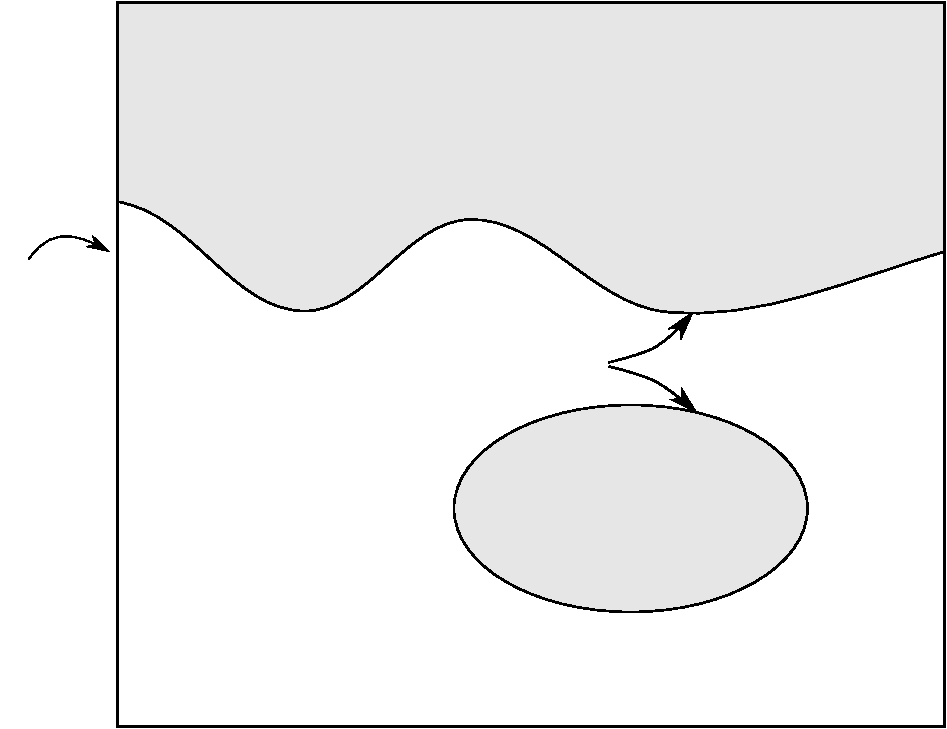
\includegraphics[width=\unitlength]{pics/sketches/domain.pdf}}%
    \put(0.62567358,0.21398357){\color[rgb]{0,0,0}\makebox(0,0)[lb]{\smash{\(\Omega_2\)}}}%
    \put(0.26114269,0.30911723){\color[rgb]{0,0,0}\makebox(0,0)[lb]{\smash{\(\Omega_1\)}}}%
    \put(0.655903,0.64519695){\color[rgb]{0,0,0}\makebox(0,0)[lb]{\smash{\(\Omega_2\)}}}%
    \put(-0.00212477,0.44771666){\color[rgb]{0,0,0}\makebox(0,0)[lb]{\(\Gamma\)}}%
    \put(0.58324946,0.3680873){\color[rgb]{0,0,0}\makebox(0,0)[lb]{\smash{\(\Gamma_d\)}}}%
  \end{picture}%
\endgroup

\caption{Skizze der Domäne nach \cite{Fries}}
\label{fig:domain}
\end{figure} 

\section{Navier-Stokes Gleichungen}
Das Strömungsfeld wird durch die Navier-Stokes-Gleichungen beschrieben, die sich aus der Masse- und Impulserhaltung ergeben. Die Herleitung soll Beispielhaft für die Massenerhaltung gezeigt werden.\\

\subsection{Massenerhaltung}

Die Massenerhaltung kann geschrieben werden als

\begin{equation}
   \DDt{M} =  \Dt \int_V \rho \id V = 0
\end{equation}

mit der Masse $M$ im Volumen $V$. Unter Anwendung des Reynolds'schen Transporttheorems und der Oberfläche $S$ des Volumens $V$ folgt daraus

\begin{equation}
    \int_V \partt{\rho} \id V + \int_S\rho(\vect{u} \cdot \vect{n})\id S = 0
\end{equation}

Durch Anwendung des Divergenztheorems können beide Terme in ein Volumenintegral zusammengefasst werden zur integralen Massenerhaltungsgleichung:

\begin{equation}
	\int_V\bigg[\partt{\rho} + \nabla \cdot (\rho\vect{u})\bigg] \id V =0
\end{equation}

Da diese Gleichung für jedes beliebige Volumen gelten muss, muss es auch
differentiell gelten:

\begin{equation}
	\partt{\rho} + \nabla \cdot (\rho\vect{u}) = 0
\end{equation}

Für inkompressible Strömungen (\(\mathrm{d}\rho = 0\)) vereinfacht sich diese Gleichung zu
\begin{equation}
	\nabla\cdot\vect{u} =0
\end{equation}


\subsection{Impulserhaltung}
Aus der Impulserhaltung folgt die differentielle Impulserhaltungsgleichung für inkompressible Strömungen nach der Herleitung in \cite{gravemeier} zu

\begin{equation}
	\partt{\vect{u}} + \vect{u}\cdot\nabla\vect{u}=\frac{1}{\rho_i}\nabla\cdot\tens{\sigma}+\vect{f}.
\end{equation}

Index $i$ unterscheidet die Größen des jeweiligen Teilgebietes. Diese Aufteilung ist nötig, da sich im Allgemeinen die Dichte $\rho$ und die dynamische Viskosität $\mu$ beider Phasen voneinander unterscheiden.

\(\tens{\sigma}\) ist der Cauchy'sche Spannungstensor und muss durch eine Konstitutivgleichung mit den Feldgrößen verknüpft werden. Im vorliegenden Fall lautet sie

\begin{equation}
	\tens{\sigma} = -p\tens{I} + 2\mu_i\tens{\varepsilon}(\vect{u}),
\end{equation}
mit \(\tens{\varepsilon}(\vect{u})
=\frac{1}{2}[\nabla\vect{u} + (\nabla\vect{u})^T]\).

\subsection{Rand- und Anfangswertbedingungen}
Für eine vollständige Problemformulierung fehlen noch die Anfangs- und Randbedingungen. Da bei den gerechneten Beispielen keine Neumann-Randbedingungen auftreten, entspricht $\Gamma$ einem reinen Dirichlet-Rand mit dem vorgeschriebenen Geschwindigkeitsvektor $\vect{g}$:
\begin{equation}
 \vect{u} = \vect{g} \auf \Gamma \times [0,T]
\end{equation}
Die Anfangswertbedingung kann geschrieben werden als
\begin{equation}
 \vect{u}(\vect{x},0) = \vect{u}_0(\vect{x}) \auf \Omega,
\end{equation}
wobei $\vect{u}_0(\vect{x})$ ein divergenzfreies Geschwindigkeitsfeld sein muss, um die Massenerhaltung zu erfüllen.


\subsection{Besonderheiten der Zweiphasenströmung}
\label{sec:twophaseflow}
% Besonderheiten der Zweiphasenströmung (-> warum XFEM?)
Die beiden Phasen sind weder ineinander löslich noch mischbar. Eine mögliche Oberflächenspannung zwischen den Phasen wird im Rahmen dieser Arbeit nicht betrachtet.\\

Am Interface zwischen den Phasen muss die Schubspannung in beiden Gebieten gleich sein, also $\tau_1 = \tau_2$. Im vorliegenden Fall wird mit dem Modell der Newtonschen Flüssigkeiten gearbeitet, weshalb gilt: 
\[\tau = \eta_i\cdot\dd{v}{y}\]
wenn $y$ die Interface-normale Richtung und $v$ die Geschwindigkeitskomponente in $y$-Richtung ist. Zusammen folgt daraus:
\[\eta_1\cdot\dd{v}{y}\biggr|_{\Omega^+} = \eta_2\cdot\dd{v}{y}\biggr|_{\Omega^-}\]

Da sich der Geschwindigkeitsgradient über das Interface ändert, entsteht an dieser Stelle ein Knick im Geschwindigkeitsverlauf. Da sich das Interface im Allgemeinen innerhalb eines Elementes befindet, lässt sich dieser Knick mit den normalen Ansatzfunktionen der FE-Methode nicht darstellen. Deshalb beschäftigen wir uns in Kapitel \ref{sec:xfem} mit erweiterten Ansatzfunktionen, die in dieser Arbeit Verwendung finden.

\section{Level-Set-Gleichung}
Zur Beschreibung des Interfaces kann entweder eine Interface Tracking- oder eine Interface Capturing-Methode verwendet werden.

Bei der Interface-Tracking-Methode wird das Interface explizit durch die
Vernetzung beschrieben, das heißt das Netz wird mit dem Interface weiterbewegt. Ein Problem dieser Methode ist, dass Topologie-Änderungen wie z.B. das Rekombinieren von zwei Blasen zu einer Größeren nicht dargestellt werden können.\\

Im vorliegenden Fall wird eine Interface-Capturing-Methode genutzt. Bei dieser wird das Interface implizit durch eine zusätzliche Feldvariable ausgedrückt. Die Änderung des Feldes unterliegt einer Konvektionsgleichung. Diese Methode lässt jegliche Art von Topologie-Änderungen zu.\\

Speziell kommt die Level-Set-Methode mit der Feldvariablen \(\phi\) zum Einsatz. Das Interface befindet sich dort bei \(\phi = 0\), es kann also als Isolinie des \(\phi\)-Feldes aufgefasst werden.\\

Die Konvektionsgleichung, mit der das Interface transportiert wird, lautet

\begin{equation}
\partt{\phi} +  \vect u \cdot \nabla\phi = 0,
\end{equation}
außerdem soll die Signed-Distance-Eigenschaft
\begin{equation}
 \phi(\vect{x}) = \pm \min_{\vect{x}_d\in\Gamma_d}{||\vect{x}-\vect{x}_d||}, \quad \forall\vect{x} \in \Omega
\end{equation} 
erfüllt werden, sodass an jedem Punkt $\vect{x}$ in $\Omega$ der Wert $\phi(\vect{x})$ den Abstand zum Interface repräsentiert. Das Vorzeichen richtet sich nach der jeweiligen Subdomäne in der $\vect{x}$ liegt. Ein positives Vorzeichen repräsentiert dabei $\Omega^+$, ein negatives Vorzeichen $\Omega^-$.

Da die Transportgleichung der Level-Set-Funktion diese Eigenschaft nicht aufrechterhält, muss in regelmäßigen Abständen reinitialisiert werden. Dabei wird über eine Funktion der Abstand von jedem Punkt in $\Omega$ der Abstand zum Interface berechnet. Zu beachten ist, dass die Funktion sehr viel Rechenzeit in Anspruch nimmt.

\section{Diskretisierung}
\subsection{Schwache Form}
Die FEM\footnote{Finite-Elemente-Methode} lässt sich schematisch mit den Schritten
\[(s) \iff (w) \approx (G) \iff (M)\]
darstellen, wobei $(s)$ die starke Formulierung aus Kapitel \ref{sec:grundlagen} bezeichnet, $(w)$ die sogenannte schwache Formulierung, $(G)$ die Galerkin-Approximation (hier ensteht der erste methodische Fehler) und $(M)$ das resultierende Gleichungssystem, das mit Methoden der linearen Algebra gelöst wird.\\

Man kann jede DGL so umstellen, dass die rechte Seite zu null wird. Die linke Seite wird dabei als Residuum $R$ bezeichnet. Diese starke Formulierung erfordert dass das Residuum an jeder Stelle im Rechengebiet $\Omega$ zu null verschwindet. Die gewichtete Residuenformulierung fordert dies, durch Integration über $\Omega$, nur im globalen Sinn:

\begin{equation}
 \int_\Omega R \id\Omega = 0
\end{equation}

Zusätzlich wird eine Wichtungsfunktion $w$ eingeführt:

\begin{equation}
 \int_\Omega wR\id\Omega = (w,R) = 0
\end{equation}

der mittlere Ausdruck stellt dabei eine vereinfachte Schreibweise der linken Seite dar, von der weiter unten wiederholt Gebrauch gemacht wird.\\

Wird in das Residuum die richtige Lösung eingesetzt, muss die linke Seite für jede beliebige Wichtungsfunktion zu null verschwinden. Wenn in der DGL eine räumliche Ableitung einer Feldvariablen vorliegt, so kann diese anschließend durch partielle Integration um eine Ordnung reduziert werden. Dadurch verringern sich die Anforderungen an die Variable.

\subsection{Galerkin-Approximation}

\subsection{Räumliche Diskretisierung der Navier-Stokes-Gleichungen}
Mit den Lösungsfunktionenräumen 
\(\mathcal{S}_{\vect{u}}\) 
für \(\vect{u}\) 
und \(\mathcal{S}_p\) 
für \(p\)
und den Wichtungsfunktionsräumen \(\mathcal{V}_{\vect{u}}\) 
für \(\vect{v}\) 
und \(\mathcal{V}_p\) 
für \(q\) 
ist eine schwache Form von \ref{} und \ref{} gegeben durch:\\ 

Finde \(\vect{u} \in \mathcal{V}_{\vect{u}}\) 
und \(p \in \mathcal{S}_p\) 
so, dass

\begin{align}
& (\vect{v},\rho\partt{\vect{u}}) + (\vect{v},\rho\vect{u}\cdot\nabla\vect{u})-(\nabla\cdot\vect{v},p) + (\varepsilon(\vect{v}),2\mu\varepsilon(\vect{u})) \nonumber\\
& \qquad = (\vect{v},\rho\vect{g}) + (\vect{v},\vect{h}_u)_{\Gamma_N} %+ (\vect{v},\gamma\kappa\vect{n}_{\mathrm{int}})_{\Gamma_{\mathrm{int}}} 
\qquad \forall \vect{v} \in \mathcal{V}_{\vect{u}} \\
&(q,\nabla\cdot\vect{u}) = 0 \forall q \in \mathcal{V}_p
\end{align}
Der Oberflächenspannungsterm, der sich bei der partiellen Integration über das Randintegral ergibt wurde weggelassen, da in den gerechneten Beispielen keine Oberflächenspannung auftritt.\\

Die Galerkin-Formulierung ist für konvektionsdominierte Gleichungen instabil und muss daher stabilisiert werden. Der Druck $p$ und die Geschwindigkeit $\vect{u}$ werden für die Diskretisierung zerlegt in 
\begin{align}
 p = p^h + \hat{p} \\
 \vect{u} = \vect{u}^h + \hat{u}
\end{align}
wobei $\hat{p}$ und $\hat{\vect{u}}$ jeweils die Anteile darstellen, die von der Galerkin-Approximation mit dem gegebenen Netz nicht aufgelöst werden. Sie werden approximiert zu
\begin{align}
 \hat{p} = -\tau_C\mathcal{R}^h_C \\
 \hat{\vect{u}} = -\tau_M\mathcal{R}^h_M
\end{align}
$\mathcal{R}^h_C$ und $\mathcal{R}^h_M$ sind die jeweiligen diskreten Residuen der Gleichungen \ref{} und \ref{}. Einsetzen dieser Zerlegung in Gleichungen \ref{} und \ref{} ergibt nach partieller Integration einiger Terme laut \cite{rasthofer} die Formulierung: Finde \(\vect{u}^h \in \mathcal{V}^h_{\vect{u}}\) 
und \(p^h \in \mathcal{S}^h_p\) 
so, dass

\begin{align}
 &\left(\vect{v}^h,\rho\partt{\vect{u}^h}\right) + (\vect{v}^h,\rho\vect{u}^h\cdot\nabla\vect{u}^h)-(\nabla\cdot\vect{v}^h,p^h)+(\varepsilon(\vect{v}^h),2\mu\varepsilon(\vect{u}^h))\nonumber\\
&\qquad+(\nabla\cdot\vect{v}^h,\tau_C\mathcal{R}^h_C)+(\rho\vect{u}^h\cdot\nabla\vect{v}^h,\tau_M\mathcal{R}^h_M)  \nonumber\\
 &\qquad= (\vect{v}^h,\rho\vect{g})+(\vect{v}^h,\vect{h}_u)_{\Gamma_N} \qquad \forall\vect{v}^h \in \mathcal{V}^h_u,\\
&(q^h,\nabla\cdot\vect{u}^h)+(\nabla q^h,\tau_M\mathcal{R}^h_M) = 0 \qquad \forall q^h \in \mathcal{V}^h_p.
\end{align}

Die zusätzlichen Ausdrücke stellen Stabiliserungsterme dar. Diese sind notwendig, da die Galerkin-FEM-Methode, bei denen die Wichtungsfunktionen den Lösungsfunktionen entsprechen, bei konvektionsdominierten Gleichungen Instabilitäten aufweisen. Zudem haben die verwendeten Lösungsfunktionen für Druck und Geschwindigkeit bei der gewählten Vernetzung die gleichen Knoten und die gleiche Polynomordnung. Die sog. inf-sup-Bedingung ist damit nicht erfüllt und daher ist ein PSPG\footnote{Pressure Stabilizing Petrov-Galerkin}-Stabilisierungsterm notwendig, der sich ebenfalls bei der Mehrskalen-Methode ergibt.

\subsection{Level-Set-Gleichung}
Mit geeignetem Lösungs- und Wichtungsfunktionenraum $\mathcal{S}_\phi$ und $\mathcal{V}_\phi$ für $\phi$ beziehungsweise $w$ lässt sich eine schwache Form schreiben als: Finde $\phi \in \mathcal{S}_\phi$ so, dass

\begin{equation}
\left(w,\partt{\phi}\right) + (w,\vect{u}\cdot\nabla\phi) = 0 \qquad \forall w \in \mathcal{V}_\phi
\end{equation}

\subsection{eXtended Finite Element Method}
\label{sec:xfem}
\subsection{Zeitintegration}

%%%%%%%%%%%%%%%%%%%%%%%%%%%%%%%%%%%%%%%%%%%%%%%%%%%%%%%%%%%%%%%%%%

\chapter{Schnittalgorithmus}

In BACI sind bereits zwei verschiedene Schnittalgorithmen implementiert. Der
gewünschte Algorithmus kann über den Parameter 

\section{Vorhandene Algorithmen}
\subsection{Tetgen}
\subsection{Hexahedra}

\section{Implementierter Algorithmus}
Da das Hex8-Element mit linearen Formfunktionen beschrieben
wird, kann das $\phi$-Feld an jeder Kante höchstens eine Nullstelle und
damit maximal einen Schnittpunkt haben.
Beim Schnitt des Interfaces mit einem Hex8-Element müssen trotzdem viele
Schnittfälle unterscheiden werden. \\

Die vielen entstehenden Schnittfälle lassen sich umgehen, indem das Hex8-Element zunächst in sechs Tetraeder-Zellen zerlegt wird und anschließend die einzelnen Tetraeder-Zellen mit dem Interface geschnitten werden. Hierbei reicht die Unterscheidung von fünf Fällen.

\subsection{Zerlegung in Tetraeder}
Es gibt mehrere Möglichkeiten einen Quader in Tetraeder zu zerlegen. Dabei entstehen entweder fünf oder sechs Tetraeder, wenn die Tetraeder nur mit den schon vorhandenen acht Knotenpunkten gebildet werden sollen.\\

Da, wie bei den Ergebnissen besprochen wird, der Schnittalgorithmus anscheinend zu einer Asymmetrie des Ergebnises führen kann, ist es von Vorteil die Zerlegung möglichst symmetrisch durchzuführen. Gerade für die quasi-2D Probleme ist es wünschenswert, dass der Schnitt auf den Flächen, die auf der Tiefenachse senkrecht stehen, jeweils gleich ist.\\

Es gibt drei Zerlegungsfälle, die diese Anforderungen erfüllen. Sie können durch 90\textdegree-Drehungen ineinander übergeführt werden. Die drei Fälle sind in Abbildung \ref{fig:cases} dargestellt. Für die Konstruktion der Tetraeder muss jede Seitenfläche in zwei Dreiecke geteilt werden. Durch die Ausrichtung der Diagonalen auf jeder Fläche sind die Schnittfälle eindeutig definiert.\\

\begin{figure}[ht]
\centering
\subfloat[Fall 1]{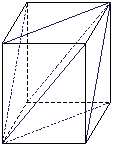
\includegraphics[width=0.25\textwidth]{pics/sketches/decomp/case1}}
\qquad
\subfloat[Fall 2]{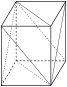
\includegraphics[width=0.25\textwidth]{pics/sketches/decomp/case2}}
\qquad
\subfloat[Fall 3]{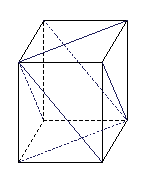
\includegraphics[width=0.25\textwidth]{pics/sketches/decomp/case3}}
\caption{Zerlegungsmöglichkeiten}
\label{fig:cases}
\end{figure}

Die Zerlegung ist in Abbildung \ref{fig:decomp} beispielhaft für \textbf{Fall 2} dargestellt: Zunächst wird der Quader in zwei Dreiecksprismen zerlegt. Anschließend können beide Prismen wie dargestellt in je drei Tetraeder aufgeteilt werden.


\begin{figure}[ht]
\centering
\subfloat[Zerlegung in zwei Prismen]{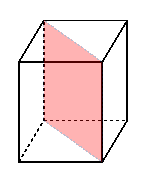
\includegraphics[height=4cm]{pics/sketches/decomp/decomposition1}}
\qquad
%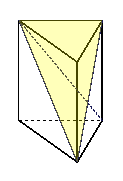
\includegraphics[height=4cm]{pics/sketches/decomp/decomposition3}
\subfloat[Hinteres Prisma in Tetraeder und Pyramide zerlegt]{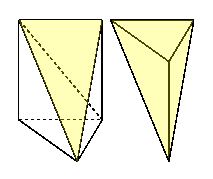
\includegraphics[height=4cm]{pics/sketches/decomp/decomposition5}}
\\
\subfloat[Pyramide in weitere zwei Tetraeder zerlegt]{
\includegraphics[height=4cm]{pics/sketches/decomp/decomposition6}}
\caption{Zerlegung in sechs Tetraeder}
\label{fig:decomp}
\end{figure}

\subsection{Schnittfälle}
Bei dem Schnitt des Tetraeders mit dem Interface werden weitere Tetraeder-Integrationszellen sowie am Interface Flächenintegrationszellen (Dreiecke) erzeugt. Zunächst werden die Schnittpunkte auf allen Kanten des Tetraeders berechnet. Wenn das Interface genau durch einen Knoten des Tetraeders verläuft, wird dies nicht als Schnittpunkt gezählt. Bis auf den Fall mit vier Schnittpunkten wird jedesmal genau eine Flächenintegrationszelle gespeichert, da der Schnitt immer eine dreieckige Fläche erzeugt. Über die Anzahl der Schnittpunkte lässt sich der Schnitt in folgende Fälle aufgliedern:

\paragraph{kein Schnittpunkt (Abbildung \ref{fig:cut0})}
Dieser Fall entspricht einer Berührung des Interfaces mit dem Tetraeder. Wenn das Element berührt wird, das heißt das Interface liegt auf einer der Seitenflächen des Quaders, wird die Zelle nicht an den Schnittalgorithmus weitergegeben. Daher kann dieser Fall nur auftreten, wenn die innere Fläche des Tetraeders berührt wird. Der Algorithmus erzeugt hier nur eine Flächenintegrationszelle.

\paragraph{1 Schnittpunkt (Abbildung \ref{fig:cut1})}
In diesem Fall geht das Interface durch zwei Knotenpunkte hindurch und teilt das Tetraeder in zwei Tetraeder.

\paragraph{2 Schnittpunkte (Abbildung \ref{fig:cut2})}
Das Interface zerlegt das Tetraeder in ein Tetraeder und eine Pyramide. Die Pyramide kann durch Teilung der viereckigen Grundfläche in zwei Tetraeder zerlegt werden. Hierbei gibt es zwei Möglichkeiten, der Algorithmus richtet sich nach der Knotennummerierung.

\paragraph{3 Schnittpunkte (Abbildung \ref{fig:cut3})} 
Zerlegung des Tetraeders in ein Tetraeder und ein Dreiecksprisma. Das Prisma kann wie im vorigen Kapitel beschrieben in weitere drei Tetraeder zerlegt werden. Es entstehen vier Tetraeder und eine Flächenintegrationszelle.

\paragraph{4 Schnittpunkte (Abbildung \ref{fig:cut4})}
Der Schnitt mit dem Interface ergibt zwei Dreiecksprismen, die wiederum in jeweils drei Tetraeder zerlegt werden. Es resultieren sechs Tetraeder und aufgrund der viereckigen Schnittfläche zwei Flächenintegrationszellen. Alternativ könnte auch ein Viereckselement (quad4) gespeichert werden.


\begin{figure}[ht]
\centering
\subfloat[kein Schnittpunkt]{\label{fig:cut0}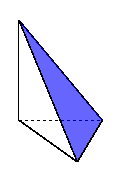
\includegraphics[width=0.2\textwidth]{pics/sketches/decomp/cut5}}
\qquad
\subfloat[1 Schnittpunkt]{\label{fig:cut1}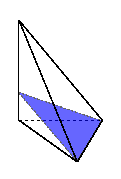
\includegraphics[width=0.2\textwidth]{pics/sketches/decomp/cut4}}
\qquad
\subfloat[2 Schnittpunkte]{\label{fig:cut2}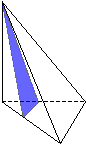
\includegraphics[width=0.2\textwidth]{pics/sketches/decomp/cut3}}
\caption{Schnittfälle I}
\label{fig:cuts1}
\end{figure}

\begin{figure}[ht]
\centering
\subfloat[3 Schnittpunkte]{\label{fig:cut3}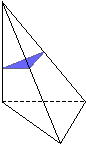
\includegraphics[width=0.2\textwidth]{pics/sketches/decomp/cut1}}
\qquad
\subfloat[4 Schnittpunkte]{\label{fig:cut4}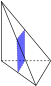
\includegraphics[width=0.2\textwidth]{pics/sketches/decomp/cut2}}
\caption{Schnittfälle II}
\label{fig:cuts2}
\end{figure}



%%%%%%%%%%%%%%%%%%%%%%%%%%%%%%%%%%%%%%%%%%%%%%%%%%%%%%%%%%%%%%%%%%

\chapter{Ergebnisse}
\section{Zalesaks-Disk}
\subsection{Problemstellung}

\def\svgwidth{0.4\textwidth}
\begin{figure}[ht]
\centering
%% Creator: Inkscape inkscape 0.48.1, www.inkscape.org
%% PDF/EPS/PS + LaTeX output extension by Johan Engelen, 2010
%% Accompanies image file 'zalesaks.pdf' (pdf, eps, ps)
%%
%% To include the image in your LaTeX document, write
%%   \input{<filename>.pdf_tex}
%%  instead of
%%   \includegraphics{<filename>.pdf}
%% To scale the image, write
%%   \def\svgwidth{<desired width>}
%%   \input{<filename>.pdf_tex}
%%  instead of
%%   \includegraphics[width=<desired width>]{<filename>.pdf}
%%
%% Images with a different path to the parent latex file can
%% be accessed with the `import' package (which may need to be
%% installed) using
%%   \usepackage{import}
%% in the preamble, and then including the image with
%%   \import{<path to file>}{<filename>.pdf_tex}
%% Alternatively, one can specify
%%   \graphicspath{{<path to file>/}}
%% 
%% For more information, please see info/svg-inkscape on CTAN:
%%   http://tug.ctan.org/tex-archive/info/svg-inkscape

\begingroup
  \makeatletter
  \providecommand\color[2][]{%
    \errmessage{(Inkscape) Color is used for the text in Inkscape, but the package 'color.sty' is not loaded}
    \renewcommand\color[2][]{}%
  }
  \providecommand\transparent[1]{%
    \errmessage{(Inkscape) Transparency is used (non-zero) for the text in Inkscape, but the package 'transparent.sty' is not loaded}
    \renewcommand\transparent[1]{}%
  }
  \providecommand\rotatebox[2]{#2}
  \ifx\svgwidth\undefined
    \setlength{\unitlength}{347.2pt}
  \else
    \setlength{\unitlength}{\svgwidth}
  \fi
  \global\let\svgwidth\undefined
  \makeatother
  \begin{picture}(1,1)%
    \put(0,0){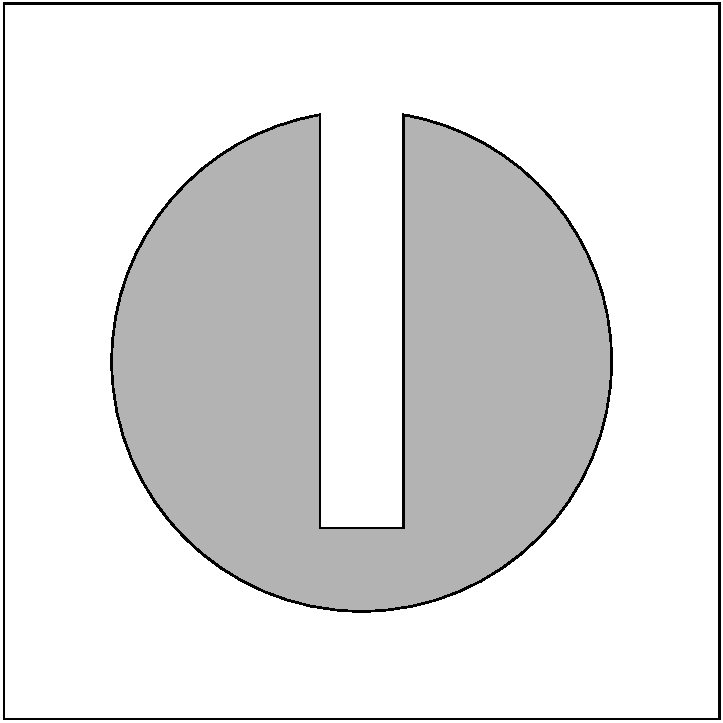
\includegraphics[width=\unitlength]{pics/sketches/zalesaks.pdf}}%
    \put(0.2764977,0.48387097){\color[rgb]{0,0,0}\makebox(0,0)[lb]{\smash{\Large$\Omega^+$}}}%
    \put(0.11520737,0.85253456){\color[rgb]{0,0,0}\makebox(0,0)[lb]{\smash{\Large$\Omega^-$}}}%
  \end{picture}%
\endgroup
\caption{Skizze des Zalesaks-Disk-Problems}
\end{figure} 

\subsection{Ergebnisse}
\subsubsection{Massenverlust}
\subsubsection{Geometrieerhaltung}

\section{Aufsteigende Blase}
\section{Rayleigh-Taylor-Instabilität}

\section{Dammbruch}
\subsection{Problemstellung}
Im Anfangszustand befindet sich eine Wassersäule($\Omega^+$) mit den Maßen $0{,}146\times0{,}292$ am linken Rand des sonst luftgefüllten($\Omega^-$) Gebietes. Das Gebiet hat die Abmaße $0{,}584\times0{,}292$. Die Materialparameter lauten: $\rho^+=\unit{1000}{\kilogram\per\cubic\meter}$, $\rho^-=\unit{1}{\kilogram\per\cubic\meter}$, $\mu^+ = \unit{$10^{-3}$}{\kilogram\per\meter\per\second}$ und $\mu^-= \unit{$10^{-5}$}{\kilogram\per\meter\per\second}$. Der Volumenkraftsvektor ist $\vect{f} = (0, \unit{-9,81}{\meter\per\squaren\second}, 0)^T$ Das verwendete Netz ist %TODO Netz.
An allen Wänden gelten Slip\footnote{Alle bis auf die wandparallelen Geschwindigkeitskomponenten werden zu null gesetzt.}-Randbedingungen. Der Zeitbereich $t = [0..0{,}25s]$ ist in 1000 Zeitschritte unterteilt.


\def\svgwidth{0.6\textwidth}
\begin{figure}[ht]
\centering
 %% Creator: Inkscape inkscape 0.48.1, www.inkscape.org
%% PDF/EPS/PS + LaTeX output extension by Johan Engelen, 2010
%% Accompanies image file 'twophaseflow.pdf' (pdf, eps, ps)
%%
%% To include the image in your LaTeX document, write
%%   \input{<filename>.pdf_tex}
%%  instead of
%%   \includegraphics{<filename>.pdf}
%% To scale the image, write
%%   \def\svgwidth{<desired width>}
%%   \input{<filename>.pdf_tex}
%%  instead of
%%   \includegraphics[width=<desired width>]{<filename>.pdf}
%%
%% Images with a different path to the parent latex file can
%% be accessed with the `import' package (which may need to be
%% installed) using
%%   \usepackage{import}
%% in the preamble, and then including the image with
%%   \import{<path to file>}{<filename>.pdf_tex}
%% Alternatively, one can specify
%%   \graphicspath{{<path to file>/}}
%% 
%% For more information, please see info/svg-inkscape on CTAN:
%%   http://tug.ctan.org/tex-archive/info/svg-inkscape

\begingroup
  \makeatletter
  \providecommand\color[2][]{%
    \errmessage{(Inkscape) Color is used for the text in Inkscape, but the package 'color.sty' is not loaded}
    \renewcommand\color[2][]{}%
  }
  \providecommand\transparent[1]{%
    \errmessage{(Inkscape) Transparency is used (non-zero) for the text in Inkscape, but the package 'transparent.sty' is not loaded}
    \renewcommand\transparent[1]{}%
  }
  \providecommand\rotatebox[2]{#2}
  \ifx\svgwidth\undefined
    \setlength{\unitlength}{506.625pt}
  \else
    \setlength{\unitlength}{\svgwidth}
  \fi
  \global\let\svgwidth\undefined
  \makeatother
  \begin{picture}(1,0.77892919)%
    \put(0,0){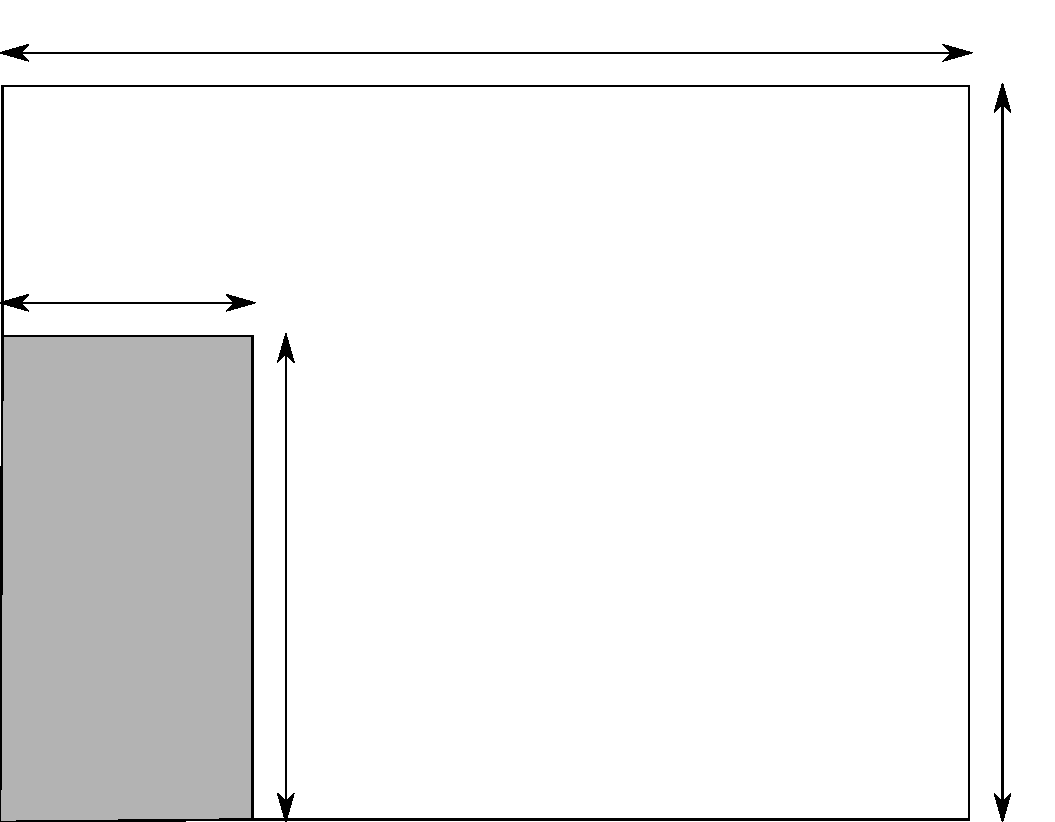
\includegraphics[width=\unitlength]{pics/sketches/twophaseflow.pdf}}%
    \put(0.39675395,0.74453491){\color[rgb]{0,0,0}\makebox(0,0)[lb]{\smash{0,584}}}%
    \put(0.96560572,0.41304281){\color[rgb]{0,0,0}\rotatebox{-90}{\makebox(0,0)[lb]{\smash{0,438}}}}%
    \put(0.05740347,0.50767333){\color[rgb]{0,0,0}\makebox(0,0)[lb]{\smash{0,146}}}%
    \put(0.28660252,0.29391038){\color[rgb]{0,0,0}\rotatebox{-90}{\makebox(0,0)[lb]{\smash{0,292}}}}%
    \put(0.09013231,0.21524025){\color[rgb]{0,0,0}\makebox(0,0)[lb]{\smash{\Large$\Omega_1$}}}%
    \put(0.57083642,0.39713792){\color[rgb]{0,0,0}\makebox(0,0)[lb]{\smash{\Large$\Omega_2$}}}%
  \end{picture}%
\endgroup
 \caption{Skizze des Dammbruch-Problems}
\end{figure}

\subsection{Ergebnisse}
\begin{figure}
 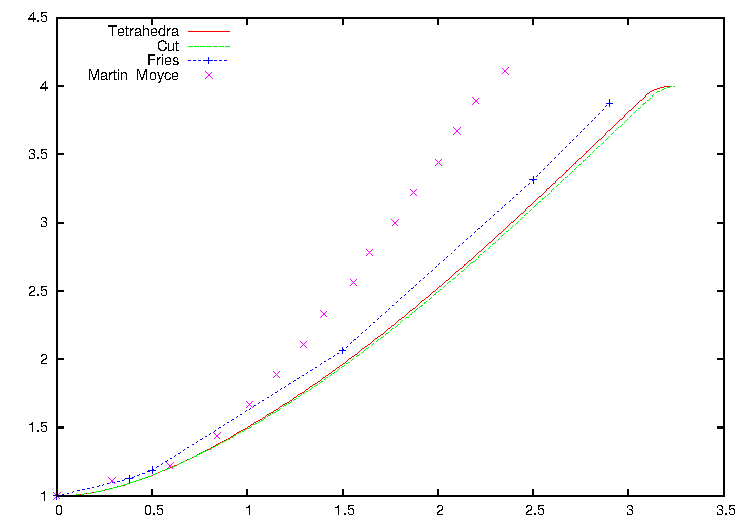
\includegraphics[width=0.7\textwidth]{pics/diagrams/plot}
\caption{}
\end{figure} 

\begin{figure}
 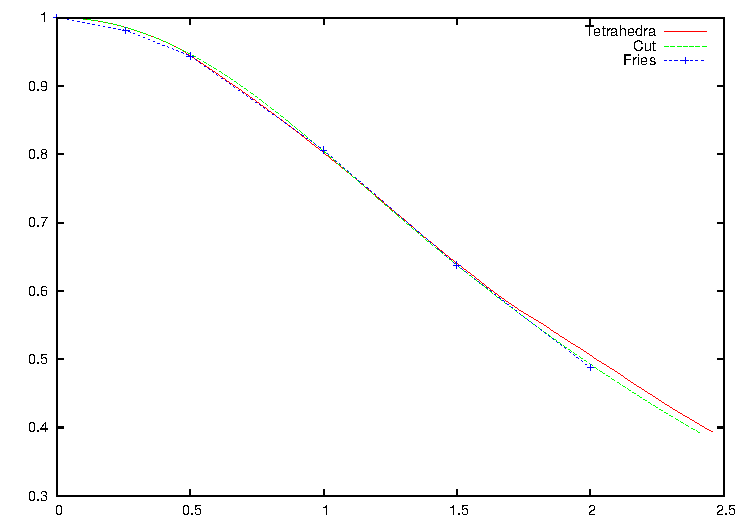
\includegraphics[width=0.7\textwidth]{pics/diagrams/plotheight}
\caption{}
\end{figure} 

%%%%%%%%%%%%%%%%%%%%%%%%%%%%%%%%%%%%%%%%%%%%%%%%%%%%%%%%%%%%%%%%%%

\chapter{Ausblick}

\appendix

\chapter{Code}
\chapter{Bilder}

\clearpage
\addcontentsline{toc}{chapter}{Literaturverzeichnis}
\bibliographystyle{plaindin}
\bibliography{books}

\end{document}

